\documentclass[conference,a4paper]{IEEEtran}
\usepackage[T1]{fontenc}
\usepackage[utf8]{inputenc}
\usepackage{amsmath,graphicx,booktabs}
\renewcommand{\abstractname}{Resumo}
\renewcommand{\refname}{Referências}
\title{Busca e otimização meta-heurística em domínios contínuos e discretos}
\author{\IEEEauthorblockN{[Nomes dos integrantes]}
\IEEEauthorblockA{Ciências da Computação --- Universidade de Fortaleza\\
Inteligência Artificial --- Trabalho AV3\\
Professor Paulo Cirillo Souza Barbosa}}
\begin{document}
\maketitle
\begin{abstract}
Este estudo avalia três buscas em cinco funções contínuas, encontra os 92 tabuleiros válidos das oito rainhas com têmpera simulada e obtém um circuito de 5359,87 unidades para 160 pontos tridimensionais com um algoritmo genético. Compara ainda quatro populações de um algoritmo genético com SBX a uma busca local aleatória em 50 dimensões sob o mesmo orçamento de avaliações.
\end{abstract}
\section{Introdução}
Em funções multimodais, movimentos locais podem convergir para extremos subótimos. Em problemas combinatórios, os operadores de busca precisam respeitar a representação das soluções. As instâncias do enunciado~\cite{av3} foram usadas para investigar esses aspectos e medir o efeito dos parâmetros.
\section{Metodologia}
\subsection{Buscas contínuas}
Minimizou-se Esfera, Ackley e Rastrigin e maximizou-se a soma de Gaussianas e a função mista. O segundo expoente da soma de Gaussianas foi interpretado como $-[(x_1-1{,}7)^2+(x_2-1{,}7)^2]$ para reproduzir a superfície exibida. Na Ackley, o segundo expoente inclui a soma dos cossenos. Na função mista, ambos os quadrados do expoente têm sinal negativo.

Hill Climbing (HC) parte do limite inferior da caixa e soma ruído uniforme em $[-\varepsilon,\varepsilon]$ por coordenada. A busca aleatória local (LRS) inicia com amostra uniforme e soma ruído normal de desvio $\sigma$. A busca aleatória global (GRS) amostra uniformemente todo o domínio a cada iteração. Os limites fixam sua distribuição, logo $\sigma$ não é ajustável. Descartam-se candidatos fora da caixa e aceitam-se melhorias estritas. Cada configuração tem 100 rodadas de até 1000 iterações e para após 250 tentativas consecutivas sem melhoria.

A grade de HC e LRS inclui 0,01, 0,025, 0,05, 0,075, 0,1, 0,15, 0,2, 0,3, 0,5, 0,75 e um valor final de 1 ou 0,99, respectivamente. Escolhe-se o menor valor testado que obtém erro objetivo de até 0,01 em pelo menos uma rodada. Se a grade falha, usa-se o menor erro mediano. As referências são zero nas três minimizações e os máximos aproximados de 2,0031167 e 2,0004500. A moda usa $f$ arredondado a duas casas e mantém empates.
\subsection{Oito rainhas}
A posição $i$ do vetor guarda a linha da rainha da coluna $i$. Maximiza-se $28-h(x)$, em que $h$ conta pares na mesma linha ou diagonal. O ótimo é 28. Cada perturbação move uma rainha para uma das sete outras linhas em sua coluna, gerando 56 vizinhos possíveis. A têmpera~\cite{kirk} aceita piora de magnitude $d$ com probabilidade $\exp(-d/T)$. A temperatura inicia em 2 e é multiplicada por 0,995 por iteração, com piso de 0,01. Cada rodada inicia aleatoriamente e para em 2500 iterações ou aptidão 28. Uma tabela hash guarda as soluções distintas. Para $I$ iterações, $R$ inicializações, $n$ rainhas e $U$ soluções, o custo é $O((I+R)n^2)$ e o armazenamento é $O(Un)$.
\subsection{Rota tridimensional}
O CSV fornece quatro regiões de 40 pontos e a origem $(0,0,0)$. Cada cromossomo permuta os 160 pontos. O custo soma distâncias euclidianas consecutivas, incluindo saída e retorno. A população tem 60 indivíduos. Torneios de três selecionam os pais. O cruzamento em dois pontos preserva um segmento de um pai por filho e preenche as posições restantes na ordem circular do outro, omitindo genes copiados. A mutação troca dois genes com probabilidade de 1\% por filho. Comparam-se zero e dois elites em 20 rodadas por configuração, com as mesmas sementes.

Como o slide 31/61 não foi fornecido, a meta é 105\% da mediana do custo final de dez pilotos independentes, cinco por configuração, com 250 gerações e sem parada por meta. Cada rodada principal para ao atingir a meta ou completar 250 gerações. A moda considera as gerações em que a meta foi alcançada.
\subsection{Comparação em 50 dimensões}
Minimizou-se $500+\sum_{i=1}^{50}(x_i^2-10\cos(\pi x_i))$. Adotou-se a caixa $[-5{,}12,5{,}12]^{50}$, pois a seção não especifica limites. O mínimo é zero na origem, já que cada parcela $x_i^2+10[1-\cos(\pi x_i)]$ é não negativa. O GA usa representação real, torneio de três, SBX com $\eta=1$~\cite{deb}, mutação gaussiana por gene (probabilidade $1/50$ e desvio 0,35), projeção na caixa e um elite. A LRS perturba uma coordenada uniforme por vez com desvio 0,8, projeta na caixa e aceita melhorias. Cada configuração tem 20 rodadas de 20 mil avaliações, incluindo a inicialização. A memória de trabalho dos estados é $O(Pn)$ no GA e $O(n)$ na LRS com dimensão $n$ e população $P$.
\section{Resultados}
\subsection{Buscas contínuas}
\begin{table}[!ht]\centering\caption{Modas de $f$ nas 100 rodadas por método}
\scriptsize\setlength{\tabcolsep}{4pt}\begin{tabular}{lrrrrr}\toprule
Função & Método & Passo & Acertos & Moda & Freq.\\
\midrule
Esfera & HC & $0{,}750$ & 94 & $0{,}00$ & 71\\
Esfera & LRS & $0{,}050$ & 6 & $0{,}00$ & 6\\
Esfera & GRS & --- & 0 & $5{,}00$ & 2\\
Gaussianas & HC & $0{,}750$ & 1 & $1{,}01$ & 52\\
Gaussianas & LRS & $0{,}010$ & 68 & $2{,}00$ & 68\\
Gaussianas & GRS & --- & 20 & $1{,}98,\;2{,}00$ & 16\\
Ackley & HC & $1{,}000$ & 0 & $0{,}10,\;0{,}15,\;0{,}22$ & 6\\
Ackley & LRS & $0{,}500$ & 2 & $0{,}15$ & 9\\
Ackley & GRS & --- & 0 & $2{,}61,\;3{,}20$ & 3\\
Rastrigin & HC & $1{,}000$ & 0 & $0{,}05,\;0{,}09,\;0{,}62,\;1{,}02$ & 3\\
Rastrigin & LRS & $0{,}500$ & 2 & $1{,}01$ & 4\\
Rastrigin & GRS & --- & 0 & $5{,}01$ & 3\\
Mista & HC & $0{,}010$ & 0 & $1{,}44$ & 100\\
Mista & LRS & $0{,}010$ & 12 & $2{,}00$ & 12\\
Mista & GRS & --- & 0 & $1{,}40$ & 5\\
\bottomrule\end{tabular}\end{table}
Na Esfera, o HC atingiu a tolerância em 94 rodadas com abertura 0,75. Nas Gaussianas, o HC aproximou o máximo em uma rodada, mas sua moda 1,01 indica concentração perto do pico local. Na Ackley e na Rastrigin, apenas a LRS atingiu a tolerância na grade testada. Na função mista, o HC ficou na fronteira inicial com abertura 0,01, e a LRS atingiu a tolerância em 12 rodadas. A escolha de passo pelo primeiro acerto favorece a menor abertura observada, mesmo quando a taxa de sucesso é baixa. As coordenadas finais e o erro mediano constam nos CSVs.
\subsection{Oito rainhas}
As 92 soluções apareceram em 1099 rodadas, com 1022 sucessos e 1005509 iterações em $3{,}47$ s. Houve 930 soluções repetidas e 77 rodadas sem sucesso. A primeira solução foi $(6, 4, 1, 5, 8, 2, 7, 3)$.
\subsection{Rota tridimensional}
A meta experimental foi $5553{,}50$ unidades. Resultados de 20 rodadas por configuração:
\begin{table}[!ht]\centering\caption{Efeito do elitismo sobre o GA de rotas}
\scriptsize\setlength{\tabcolsep}{4pt}\begin{tabular}{lrrrrr}\toprule
Elites & Aceitas & Moda & Freq. & Melhor & Mediana\\
\midrule
0 & 15 & 227 & 2 & $5359{,}87$ & $5527{,}95$\\
2 & 7 & Empate & 1 & $5498{,}94$ & $5810{,}23$\\
\bottomrule\end{tabular}\end{table}
Sem elitismo, a geração 227 ocorreu duas vezes entre os 15 sucessos. Com dois elites, as sete gerações bem-sucedidas foram 109, 117, 123, 128, 131, 152 e 212, uma ocorrência cada. O elitismo não se mostrou necessário nesta configuração. Embora preserve os melhores indivíduos de uma geração, pode reduzir a diversidade. Os experimentos mediram o efeito final sobre as rotas, sem medir a diversidade diretamente.
\begin{figure}[!ht]\centering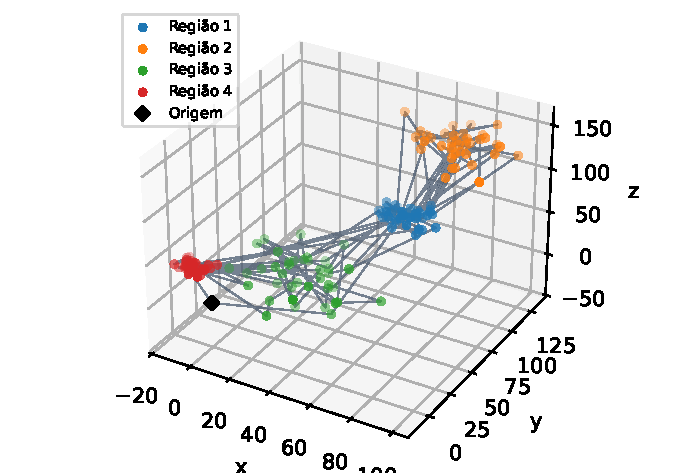
\includegraphics[width=.68\columnwidth]{rota.pdf}\caption{Melhor circuito encontrado. O marcador preto indica a origem.}\end{figure}
\subsection{Comparação em 50 dimensões}
\begin{table}[!ht]\centering\caption{Qualidade e tempo por rodada em 50 dimensões}
\scriptsize\setlength{\tabcolsep}{4pt}\begin{tabular}{lrrrr}\toprule
Método & $P$ & Melhor & Mediana & Tempo (s)\\
\midrule
GA-SBX & 20 & $161{,}145$ & $185{,}922$ & $0{,}136$\\
GA-SBX & 50 & $115{,}420$ & $174{,}014$ & $0{,}094$\\
GA-SBX & 100 & $141{,}252$ & $210{,}601$ & $0{,}065$\\
GA-SBX & 200 & $285{,}890$ & $367{,}748$ & $0{,}063$\\
LRS & --- & $0{,}022$ & $0{,}056$ & $0{,}173$\\
\bottomrule\end{tabular}\end{table}
O GA com 50 indivíduos apresentou a menor mediana entre os GAs e menor tempo médio que o GA com 20 indivíduos. As populações 100 e 200 terminaram mais rápido, mas com medianas piores. Sob orçamento fixo, elas renovaram a população menos vezes. A LRS obteve o menor custo final com memória de trabalho linear. A função é separável, o que favorece o ajuste de uma coordenada por vez. Nesta implementação, o tempo médio da LRS foi maior, em parte porque o GA avaliou lotes em NumPy.
\begin{figure}[!ht]\centering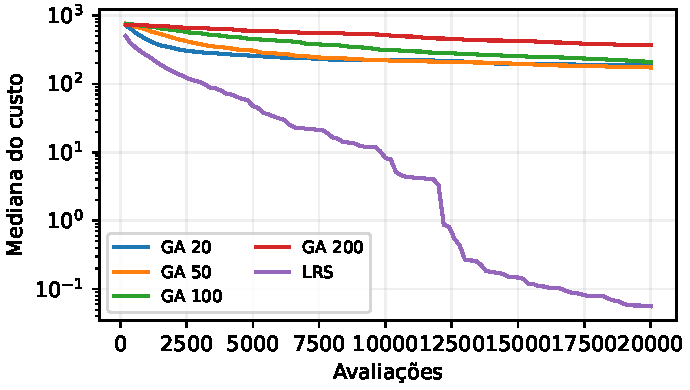
\includegraphics[width=.84\columnwidth]{convergencia.pdf}\caption{Mediana do melhor custo por orçamento de avaliações em 50 dimensões.}\end{figure}

\section{Conclusões}
Nas buscas contínuas, um acerto ocasional coexistiu com modas distantes do ótimo. A têmpera obteve os 92 tabuleiros após reinícios e revisitas. No caixeiro, o GA sem elitismo atingiu a meta em mais rodadas e obteve a menor distância. A comparação em 50 dimensões quantificou o efeito do tamanho de população sob um orçamento fixo. Os hiperparâmetros e a meta do caixeiro dependem da instância e do orçamento experimental.
\begin{thebibliography}{00}
\bibitem{av3} P. C. S. Barbosa, \emph{Trabalho AV3 --- Busca/Otimização Meta-heurística}, Universidade de Fortaleza, 2026.
\bibitem{kirk} S. Kirkpatrick, C. D. Gelatt Jr. e M. P. Vecchi, Optimization by simulated annealing, \emph{Science}, vol. 220, pp. 671--680, 1983.
\bibitem{deb} K. Deb e R. B. Agrawal, Simulated binary crossover for continuous search space, \emph{Complex Systems}, vol. 9, pp. 115--148, 1995.
\end{thebibliography}
\end{document}
